% easychair.tex,v 3.5 2017/03/15

%\documentclass{easychair}
\documentclass[EPiC]{easychair} % this is for ISCA conference proceedings
%\documentclass[EPiCempty]{easychair}
%\documentclass[debug]{easychair}
%\documentclass[verbose]{easychair}
%\documentclass[notimes]{easychair}
%\documentclass[withtimes]{easychair}
%\documentclass[a4paper]{easychair}
%\documentclass[letterpaper]{easychair}

\usepackage{doc}

%
\newcommand{\easychair}{\textsf{easychair}}
\newcommand{\miktex}{MiK{\TeX}}
\newcommand{\texniccenter}{{\TeX}nicCenter}
\newcommand{\makefile}{\texttt{Makefile}}
\newcommand{\latexeditor}{LEd}


\title{How to pimp legacy enterprise content management systems and successfully run them in the cloud
    \thanks{Other people who contributed to this document include Gang,Shao and Pascal,Hirmer (The University of
  Manchester).}}

% Authors are joined by \and. Their affiliations are given by \inst, which indexes
% into the list defined using \institute
%
\author{ Cataldo Mega\inst{1}\thanks{Designed and implemented the class style}}

\institute{ University of Stuttgart, Stuttgart, BW, Germany\\\email{cataldo.mega@ipvs.uni-stuttgart.de}}

\authorrunning{Mega, at al }

\titlerunning{The {\easychair} Class File}

\begin{document}

%\maketitle

\begin{abstract}

  If you care about your legacy ECM system, it's a natural step to want to take the specifics of your system into your own hands. Modifying or "pimping" out your ECM system does not have to be an open-ended process. Most enterprises want to soup up the end-user look and feel and add practical improvements to their ECM system brewing a healthy mix of both. Although modification can be expensive in the end an over-haul can vastly increase the value and boost your business.
 
  \paragraph{} ECM systems are the custodian of unstructured data employing the corporate information life cycle and governance strategy supporting records management and legal e-discovery. As such, ECM systems are the common corporate document repository and enterprise archive. Over the last decades legacy ECM production environments and related application development, test and provisioning processes have become slow, inflexible and too expensive in order for being competitive with cloud native solutions. However, there is a remedy to this. Our investigations show that it is possible to overcome the shortcomings of the current legacy systems architecture design and to close the gaps by evolving the old client server computing into a modern cloud-computing models.
  For our investigations we re-implemented a prototype ECM systems for running it on a cloud platform such for being able to compare it against the classical approach. The focus of our analysis was on understanding aspects of run time environment preparation, setup, component configuration and finally deployment. We found that design pattern used in a client-server computing model have become anti-pattern in a cloud-computing world, thus preventing the exploitation of new cloud platforms. Despite of this findings we show that by applying right corrective measures it is possible to pimp a legacy ECM system and successfully run them in the cloud.        
  
  \paragraph{Keywords.} Enterprise content management, architecture design, cloud-computing model.
  
\end{abstract}

%------------------------------------------------------------------------------
\section{Introduction}
\label{sect:introduction}

Cloud computing has become synonymous with a faster, scaleable, flexible and cost efficient IT-Infrastructure offered as a service on-line. Influenced by these promises CTO's in companies are driving the restructuring of their ECM IT-Environment as the legacy development,test and provisioning processes have become slow, inflexible and expensive. These circumstances led to an erosion of competitiveness against cloud native solutions. On the other hand, what has been working well for years and where substantial investments have been made can't be thrown over-board just like this. Therefore the challenge is to find out how a content management as a service – CMaaS  offering can be created tailored for the B-B Eco-system in which to build quickly an attractive and profitable food chain with an enhanced legacy ECM systems.

In order to develop possible strategies to solve these problems it important to understand what the problems . The questions we asked to ourselves were, i) is it possible to evolve the old legacy ECM systems design and ready it for the ‘Cloud’ or ii) is it better to slowly phase it out and replace the legacy with a cloud native version.

\textbf{Goals.} 
In order to understand how to achieve our goals, we investigated the architecture design changes required to cloud enable content management solutions by analyzing their workloads related to document management, compliance archiving, records management and e-discovery. Our approach was to determine the shortcomings of the legacy client-server computing model employed that prevents the transition into cloud-computing world. In a second step, we want to develop strategies on how to evolve the current architecture design and prove with a prototype implementation that with the exploitation of cloud technology is it possible to compete successfully against the new cloud native applications in the ECM market place. 
%------------------------------------------------------------------------------

\section{Foundation}
\label{sect:foundation}

Throughout this document we use the term content for unstructured data of any type and format created, changed or used inside a company and which is considered important enough for being put under control of the information life cycle management (ILG) system as mandated by corporate governance policies.” Think of ECM as a data warehouse system for unstructured content.

\paragraph{}   Every enterprise is obliged to implement an information life cycle based on a governance model that ensures information is properly handled, based on business context and in order to comply with corporate governance policies and legal regulations. In practice, enterprises have a dedicated infrastructure in place to manage the life cycle of content produced by their business applications, business processes and to satisfy their business intelligence needs. Enterprise content management is therefore the governance practice to handle the of the information life cycle in a heterogeneous, geographically distributed corporate data landscape and ultimately the actual motivation behind the existence of ECM Systems. The entirety of business applications builds the company application portfolio, which in turn produces the data specific to the services they provide. 

\paragraph{} The implied work processes collect and gather product related information, collateral materials about involved entities as required by the business corporate and legal compliance. One can imagine these applications being part of a highly integrated and interconnected application framework where data flows from source to sink using guarded and secured data pathways through a corporate data hub as outlined in figure 2 below

\paragraph{} The ECM system design shown above follows an application model employing a multi-tier architecture consisting of layers the client, the Web, the application, the data access, and the storage layer at the lowest level. The lower part of figure 2 can be thought of being the back plane of the application portfolio represented by legacy databases, data warehouses and complemented by the ECM system with its content management services. It is below the common content services layer where the management of the enterprise information life cycle (ILG) takes place. ILG is synonymous for “Services build to manage all business relevant content which is collected, indexed, annotated, classified, stored, archived and finally disposed as mandated by the corporate governance policies	.”

\textbf{Definition:} In the enterprise content management context we use the term content to refer to any kind and any type of unstructured business data, be it in form of office-documents, files, images, audio, video or any other multi-media content. Often we will call them ‘content objects’ or simply ‘content’ or ‘objects’. 

\textbf{Definition:} In the enterprise content management context we use the term ‘meta-data’ to refer to information about the ‘content’ its relation to the business it belongs to and the required management and operational information to support the corporate information life cycle, governance and compliance processes. 

Meta-data refers to structured data, meaning relational data managed through a relational database management system (RDBMS). Additionally, full-text indexes and more recently, modern AI and ML knowledge bases complement the relational meta-data index. In the end, meta-data serve the purpose for an efficient information retrieval end user experience.

\subsection{2.1	What is the purpose of content management in an enterprise}
The need for a content management system becomes obvious when considering the answers to the following questions:

\begin{enumerate}
    \item 1.	What kind and type of data exists and is available in my company?
    \item 2.	Where is the data coming from, and where is it stored? 
    \item 3.	Is the data classified, categorized and properly secured?
    \item 4.	Who is the responsible custodian of the data? 
    \item 5.	Who needs or is authorized to access what information or data? 
    \item 6.	How long must the information be retained and when is it due to be disposed?
    \item 7.	How can the data be imported, made available internally and exported as required?
\end{enumerate}

Answering these questions lead to the specification of business requirements and the definition of the information life cycle and governance (ILG) strategy, which in the end enforces the existence of an enterprise content management system. 

\paragraph{}  At its core, the ILG strategy implies that for every piece of relevant business data there must exist an audit record at any given time, such to withstand internal and external audits. The totality of these records represents the foundation of an enter-prise ‘content information catalog’. The content information catalog, the logic that drives the unstructured information life cycle and the repository facilities required to manage the physical content represents the actual ECM system.

\subsection{ How is content managed in an enterprise? }
At the very least, an ECM system consists of a data catalog, one or more content repositories and the facilities for users and application to access the system. Technically speaking the enterprise data catalog can be thought of a relational schema having 3 distinct sections: i) the business related document model, ii) the administrative data model and iii) the operational data model. 

\paragraph{} A special subset of the operational model can be seen as a set of ‘content-object locators’, basically references to every piece of physically stored content in repositories located and managed somewhere in the company.  Stored content and their references are kept always in sync such to avoid dangling pointers and orphaned objects keeping referential integrity between the metadata in the central catalog and the actual digital content in the associated content repositories. The technical implication is that an ECM system must ensure strict consistency between the central catalog and the slave content repositories. A required prerequisite for this to happen is the implementation of transactional integrity between the master and its slave servers using a 2-phase commit protocol. Together the content catalog, the management component, the business support, storage administration components, the workflow engine and infrastructure required to keep the processes going, constitute the ‘Enterprise Content Management’ Application System.

\subsection{Definition of enterprise content management }

The Association for Information and Image Management (AIIM) defines Enterprise Content Management as follows: [AIIM 2020] “Enterprise Content Management is the systematic collection and organization of information that is to be used by a designated audience – business executives, customers, etc. Neither a single technology nor a methodology nor a process, it is a dynamic combination of strategies, methods, and tools used to capture, manage, store, preserve, and deliver information supporting key organizational processes through its entire life cycle. ”   

\paragraph{} My conclusion is that the relation between enterprise content management and in-formation life cycle (ILG) is that the ECM implements the ILG as a combination of strategies, methods, and tools used to handle all relevant information required to run an enterprise in an appropriate and legal way.

\subsection{Then what is enterprise content management all about?. }

We learned that, all documents and materials created or processed in the course of a business conducted by a company, if deemed relevant is kept for as long as it is required to comply with corporate and legal compliance. This means that from a technical standpoint ECM Systems consists of a collection of IT-infrastructure components that fit into a multi-layer model for efficiently managing the information life cycle and governance (ILG) of unstructured data in a company. The enterprise wide, successful implementation of an information life cycle that supports the key organizational business processes is what defines a valid enterprise content management strategy. In the end, if data is the fuel then the ECM system is the fuel tank and the logic that supports the available business engines.

\paragraph{} In summary, what the business needs from an ECM systems is that:
\begin{itemize}
    \item Content must be located, pre-classified, captured, ingested and persisted in an automated fashion,
    \item Content must be easy to be searched, found, and identified
    \item Content must be efficiently index independent of type and format 
    \item Access must be secure, transparent and fast 
    \item Information 	retrieval should be comprehensive, accurate and available at any-time from anywhere.
    \item Content has to obey corporate and regulatory compliance
    \item Support for corporate litigation and case management should be provided 
    \item Content output and delivery must be flexible, fast and secured 
\end{itemize}

\subsection{But where is all the content stored in an enterprise?}

Employees and application processes manage, control and store documents, files and content they own typically on network drives. Alternatively office documents are
stored online in an Office365 or MS SharePoint site used as an active unstructured data repository. Once a document reaches its final, immutable state it is loaded into save harbor which takes over the responsibility to enforce its intended life cycle. Usually this is ‘the ECM system’. 

\paragraph{} While in the ECM system the content is managed, controlled and stored in several content repositories where individual content objects are physically stored on storage devices, be it a simple a file systems or a sophisticated hierarchical storage management systems that includes optical and tape subsystems. Recently content is increasingly also stored cloud drives. 

\paragraph{} The common link among content repositories is the presence of a common object access and management layer (OAML), which represents the software component that unifies seamless content object operations like store, update, retrieve delete, de-duplicate, encrypt, migrate and replicate. Our experience taught us that in one way or another every company has its version of an ECM system in place. 

\paragraph{} The more complex ECM systems are within multi-national companies like multi-national banks, insurances, and pharmaceutical or logistics companies. Their ECM systems span across countries and all over the world. The fact of acting at a multi-national level poses an even higher burden to firms as this means that they have to cope with larger amounts of data and from many different jurisdictions. For an enterprise, this means it has to entertain a quite large IT-infrastructure distributed over geographically dispersed locations and that might cross country borders. Therefore, there are many costs associated with the different aspects of keeping product development, test and production systems up and running when it comes to roll-out product releases and to keep production smoothly rolling. 

\paragraph{} Considering what we explained before it becomes clear why higher management in a company asks the following questions: 

\begin{itemize}
    \item Can we boost productivity at a faster pace?
    \item Can IT-capital investment be changed in capital expenditure?
    \item Can administration and operations cost be reduced?  
    \item Is it possible to grow business with the same IT-personnel?
\end{itemize}

\paragraph{}  Our investigations and analysis indicates that there are positive answers to those questions.
%------------------------------------------------------------------------------
\section{Related Work}
\label{sect:relatedwork}

Related work goes in here  …. Was gibt es was andere schon gemacht haben 

\begin{enumerate}
    \item 1st item
\end{enumerate}

%------------------------------------------------------------------------------
\section{Business and corporate requirements on content management}
\label{sect:business-requirements}

In the context of the overall enterprise information management (EIM) the set of content management services, represent the subset of EIM services related to unstructured data. Therefore, in this paper, we use the terms enterprise information management and enterprise content management synonymously, but with a focus on content management. 

\paragraph{} In typical production environment ECM systems integrates with the company’s back-office systems, file servers and email archives representing the majority of sources of business data and collateral materials. Through specific integration points, relevant information is collected based on collection policies mandated by corporate policies. Classification of electronic assets in to ‘business relevant’ or ‘disposable after use’ happens at the data sources. All the business relevant assets are then captured and digitally transferred to the enterprise content repository for subsequent use. 

\paragraph{}
Using [AIIM 2020] definition, ECM systems do store and manage the common in-formation, documents and multi-media content that the business produces directly or indirectly and supports the enterprise information life cycle and governance strategy relative to unstructured data. This means, business applications and corporate governance can be satisfied by the following business requirements:
\begin{itemize}
    \item BR-01. Collect, ingest and store business relevant information, data and materials of any type and format.
    \item BR-02. Support classification, categorization and tagging of information relevant to business, corporate and legal.
    \item BR-03.  	Allow efficient indexing, search and retrieval of information 
    \item BR-04.  	Provide metadata management and data modeling facilities for sup-porting enterprise document management and archiving 
\end{itemize}

\paragraph{} The above listed business requirements helps us derive the functional requirements and to define system component capable for satisfying the business needs.

\subsection{ Functional requirements by workload type} 
\begin{itemize}
    \item FR-01. Collect, capture and ingest of unstructured data
    •	This component comes as a set of crawlers, collectors and loader tasks that automatically scan through file systems over the network, crawl Web sites or access mail systems in search for qualifying information. By doing so, valuable data is collected and loaded in to the content repository for further processing and use. We refer to these services as ‘Content Collection or Data Input or Capture’ services
    \item FR-02. Content classification of unstructured data \paragraph{} This component is responsible for classifying information, documents and con-tent collections based on corporate and legal taxonomies after being loaded in-to the content repository.
    \item FR-03. Information governance services. \paragraph{} Governance is synonymous with ‘having in place the required tools and processes used to enforce enterprise and legal compliance’. Governance is based on given classification libraries and relative taxonomies that define the security, privacy policies, retention and disposition rules applied to captured information.
    \item FR-04.Content output and delivery to internal and external recipients \paragraph{} Information designated for delivery out of the enterprise repository to internal and external location in a secured, fast and flexible. The service includes for-mat conversions, encryption, packaging and delivery capabilities using push, pull and streaming methods over the network. 
    \item FR-05. Content management and enterprise repository services \paragraph{} This is the core of content management. It consists of a system wide central data catalog that comes with a predefined repository schema, addressing authentication, authorization, management as well as aspects of security and compliance. Business applications and external services integrate with the system catalog by enhancing and complementing the system schema and repository logic. The data catalog exposes relational metadata based search and retrieval services, complemented with content based full-text search capabilities. 
    \item FR-06.Document management services \paragraph{} The integration of business departments, Line of Business (LoB) applications, the back-office and others happens by mapping sub-sets of the application document models into the ECM master catalog and the implementation is through the publishes repository APIs. 
    \item FR-07. Information archive services \paragraph{} Information, documents and electronic artefacts are kept under control for long term archiving. The information assets are associated with the necessary document model built of index data in the data catalog and made ready for search and retrieval. The physical assets are stored on storage devices according to content type specific retention's policies. As they age, they are migrated through a storage hierarchy before being disposed after reaching the end of their life cycle.  
    \item FR-08. Support for the information life cycle and governance services. \paragraph{} The governance services provide support for the information life cycle governance, realized by means of a catalog schema enhancement, the provisioning of access control policies, the rules specifying where and how to store information assets and their defensible disposal at the end of the life cycle
    \item FR-09. Support for content centric workflows services \paragraph{} The ECM repository uses a content centric workflow engine for document routing tasks such as the approval process of a loan application or an insurance claim application.
    \item FR-10. Records management, hold and preservation services \paragraph{} Corporate and legal obligations require the application of security, privacy and retention policies for all information, documents and electronic artefacts under the custody of the enterprise repository. 
    \item FR-11. Support for legal case and e-Discovery services  \paragraph{} In case of a legal dispute, involved content collections must be put on hold until the case is closed. E-Discovery relates to a more sophisticated search and retrieval process, requiring that unstructured data is full text indexed and tagged with legally relevant information meant to aid the e-discovery service in finding and putting a legal hold on case relevant documents. 
    \item FR-12.Content object and storage management services \paragraph{} The component is the ECM Resource Manager (RM) or Object Server (OS). Its constituent sub-components consists of a database schema with references to the physically stored objects, the information related to storage management and an elaborated logic that implements the storage management functions. The storage management service includes hierarchical storage management, content transformation and movement services. If required content is de-duplicated, encrypted, rendered, transcoded, migrated and replicated based on business need. In the end, content it is always disposed meaning deleted in a legally defensible way. Resource Managers depend on the master catalog that plays the role of a transaction coordinator responsible for ensuring referential integrity. The work location of Resource Managers is near to the audience where the stored information is mostly required, or imposed by jurisdictions or cost.
\end{itemize}

\subsection{Non-functional requirements for ECM systems} 

\paragraph{} By experience performance and scaleability, requirements are integral part of the system design. For ECM system, a major focus is on how efficiently it can handle an unknown and variable number of documents, ingested at highly variable rates by a possibly very large population of end users and external sources. Additionally, the ingested content triggers the indexing process creating the required search index such to expedite retrieval and minimize time delays. 

\paragraph{} The following list shows the key non-functional requirements for the ECM systems:

\begin{itemize}
    \item NFR-01. Keep strict referential integrity between meta-data and data avoiding dangling pointers and orphan objects.
    \item NFR-03. Cope gracefully with load variations minimize system disruptions such to ensure high availability and resilience to outages. 
    \item NFR-04. Dynamically adapt the production-environment to current load variations by proper handling the commissioning and decommissioning of IT resources.
\end{itemize}

%------------------------------------------------------------------------------

\section{ECM systems architecture and implementation design}
\label{sect:architecture-design}
\subsection{ECM architecture blueprint }

At the high level the ECM systems architecture exposes five key system layers.

\begin{enumerate}
    \item  End-user, devices and presentation layer
    \item  Content services layer
    \item  Content management and repository layer
    \item  Content resource management layer
    \item  Object storage management and access layer 		
\end{enumerate}

which are visualizing in the next figure.

 \begin{figure}[hbt!]
     \centering
	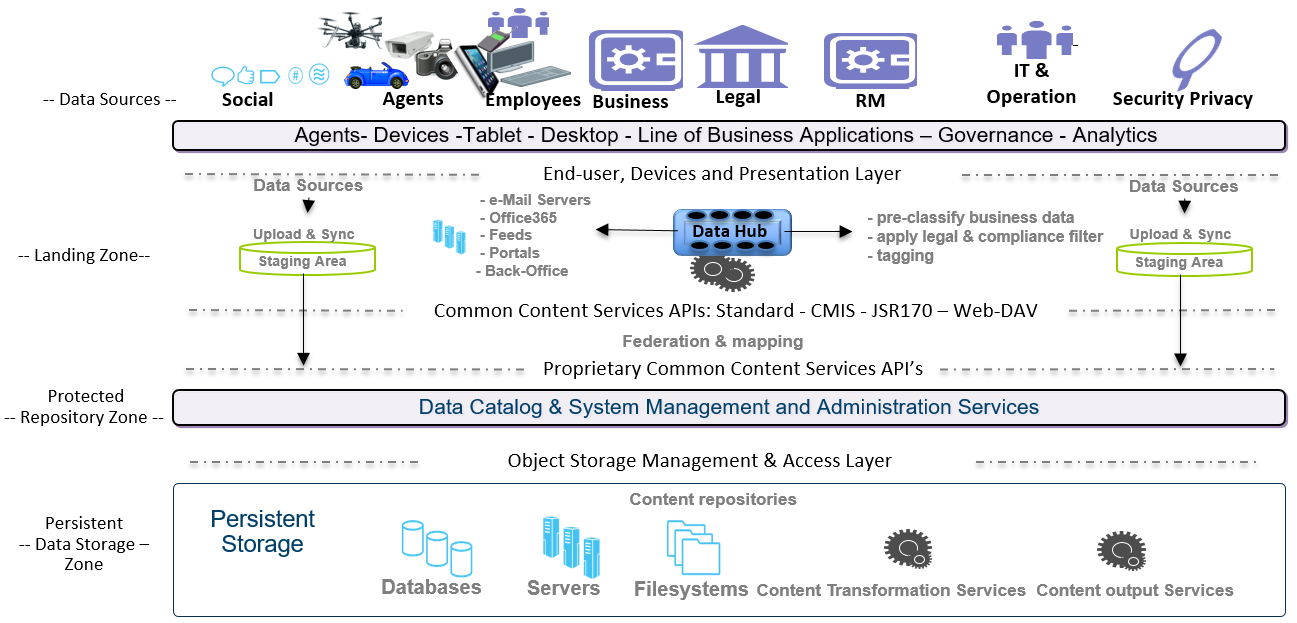
\includegraphics[width=0.5\textwidth]{pics/ECMpic03}
     \caption{ECM architecture blueprint showing components by layer}
     \label{fig:architecture-blueprint}
 \end{figure}

Figure 3 outlines a widely accepted blueprint of a ECM system architecture, showing the five layer and the respective functional components in that layer. In this pa-per, I am restricting the design analysis to the core ECM components at the ‘Content management and repository’, the ‘Content resource management’ and the ‘Object storage management and access’ layers.

\subsection{Enterprise content management and repository services layer. }

This layer hosts the core ECM services accessible through the ECM repository APIs. 

\begin{figure}[hbt!]
	\begin{centering}
%	
\includegraphics[width=0.5\textwidth]{logoEC}
	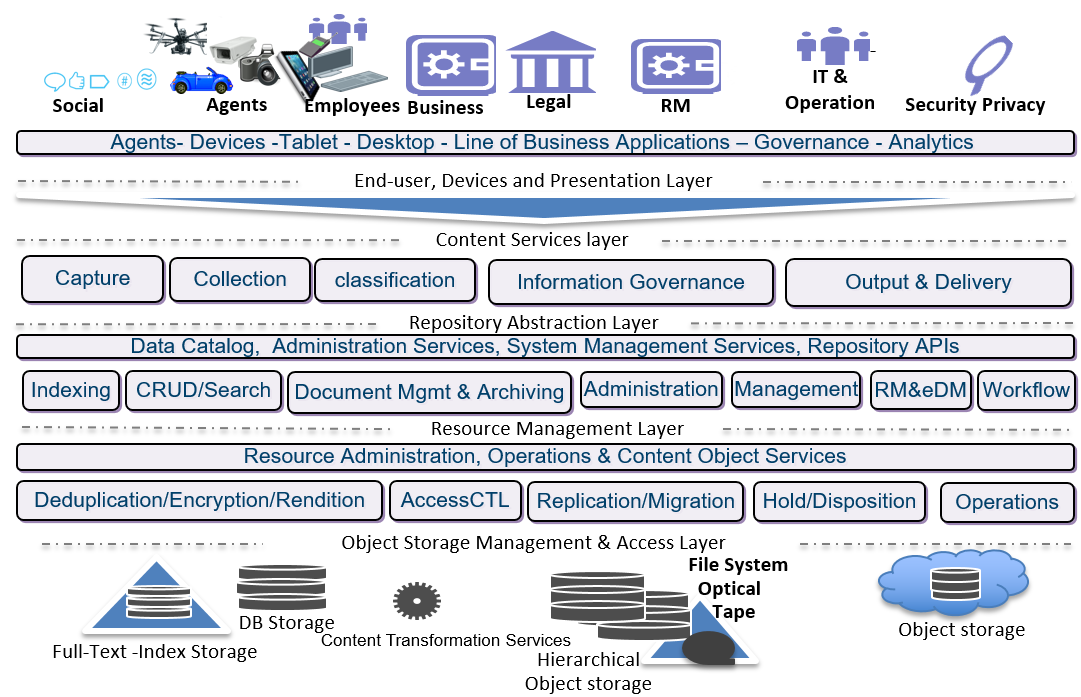
\includegraphics[width=0.5\textwidth]{pics/ECMpic04}
	\caption{Components of the content management and repository layer}
	\label{fig:ecm-components}
	\end{centering}
\end{figure}

\paragraph{} The whole repository concept relies on the existence of a central catalog the master and one or more dependent but decentralized content repositories the workers. This approach was chosen due to the implementation of the ‘separation of concerns’ software design principle. 

\paragraph{} In practice, this means to keep the administration of the many physical content independent of the central meta-data catalog and to separate meta-data management from physical content management. The benefit by doing so, is that accessing a document via the central catalog is completely agnostic from where the document is physically located. Access to a the stored electronic object becomes transparent from its physical location even if that object is physically moved from one storage device to another or from one location to another. 

\paragraph{} Think of corporate archive policies mandating that content storage locations and access control depends on document type and state and thus change over time. But end-users do not have to worry from where a document is coming from as long as it is accessible.

A short list of the components in the content management and repository layer are:

\begin{enumerate}
    \item •	Core ECM APIs – ECM repository APIs available are standard, proprietary and federated APIs. All support transparent repository wide execution of primitive CRUD functions, search and retrieval as well as hold and disposal operations.
    \item •	Data catalog and modelling services – The ECM system catalog expands over a number of decentralized distributed databases working together in a master-worker relationship as outlined in figure 6.

\begin{figure}[hbt!]
	\begin{centering}
%	
\includegraphics[width=0.5\textwidth]{logoEC}
	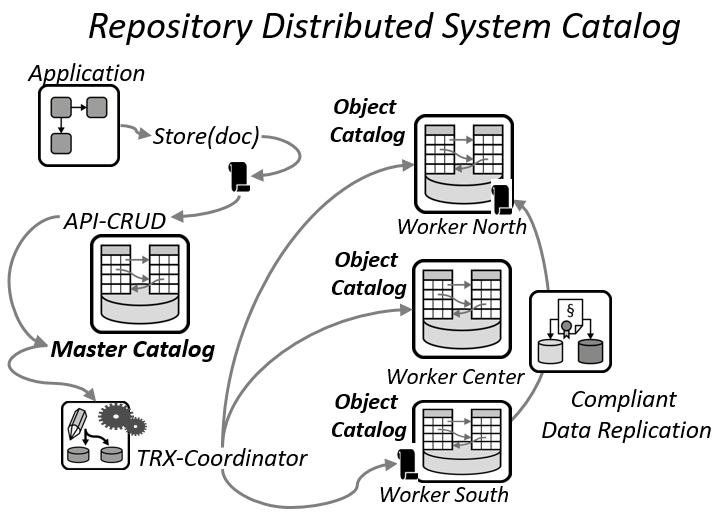
\includegraphics[width=0.5\textwidth]{pics/ECMpic06}
	\caption{ECM system catalog implemented as a set of distributed databases}
	\label{fig:ecm-catalog}
	\end{centering}
\end{figure}

\paragraph{} Fig. 6. ECM system catalog implemented as a set of distributed databases
The master or central catalog implements a flexible relational schema on top of a scaleable database system. It comes armed with a predefined entity relationship model with a set of repository entities, associated metadata and functional dependencies.  ECM applications typically define their specific document model extensions implemented using the repository modeling APIs. The API layer in turn for mapping the data model it into the overall relational schema The integration with line of business applications (LOB) is realized through the system data modeling capabilities where a flexible blend of customer and system entities can be created together with associated business logic. Figure 7 provides a simplified view of the application integration points.

\begin{figure}[hbt!]
	\begin{centering}
%	
\includegraphics[width=0.5\textwidth]{logoEC}
	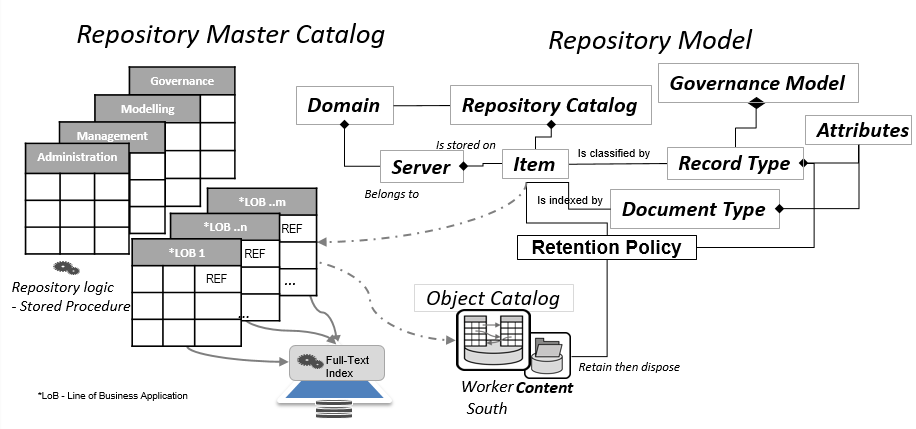
\includegraphics[width=0.5\textwidth]{pics/ECMpic08}
	\caption{Application integration points as exposed by the ECM system catalog}
	\label{fig:ecm-system-catalo}
	\end{centering}
\end{figure}

    \item •	Indexing, search and retrieval services – The information retrieval services sup-ports relational and full text indexing as well as search and retrieval of information aided by database and full-text-indexes via an integrated FT-Engines.

\begin{figure}[hbt!]
	\begin{centering}
%	
\includegraphics[width=0.5\textwidth]{logoEC}
	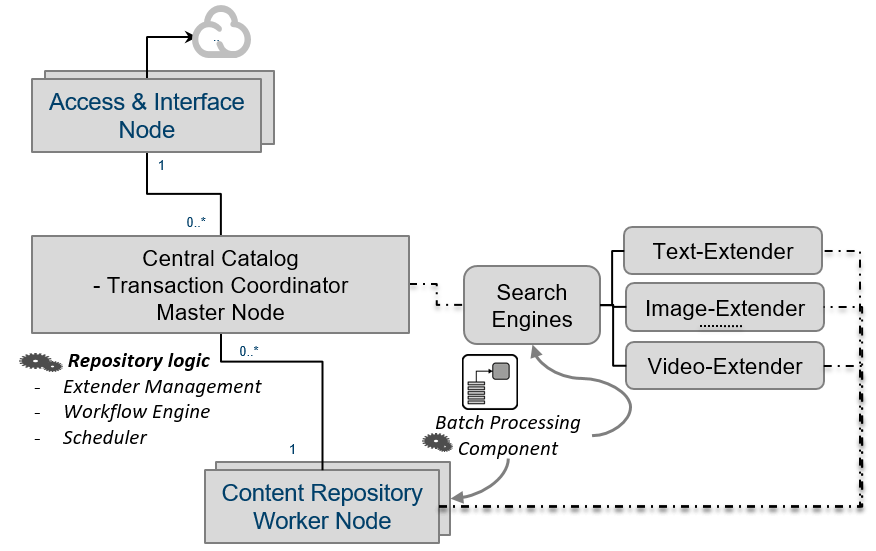
\includegraphics[width=0.5\textwidth]{pics/ECMpic09}
	\caption{Search engine Integration with ECM system}
	\label{fig:ecm-search-engine}
	\end{centering}
\end{figure}

    \paragraph{} Line of business application integrate with the basic repository data model by ex-tending it with application specific sub-schema, such for being able to persist application metadata the relational index which later is used to search for and retrieval of meta-data relative to unstructured data objects stored in the repository. Usually, a distributed cluster of full text indexes complements the relational schema. Thus, their full text search companions complement the relational searches.
    
    \item •	Information life cycle and governance (ILG) support services – enforce enterprise governance policies by configuring and monitoring a category specific, secured information life cycle from ingestion to destruction.

\begin{figure}[hbt!]
	\begin{centering}
%	
\includegraphics[width=0.5\textwidth]{logoEC}
	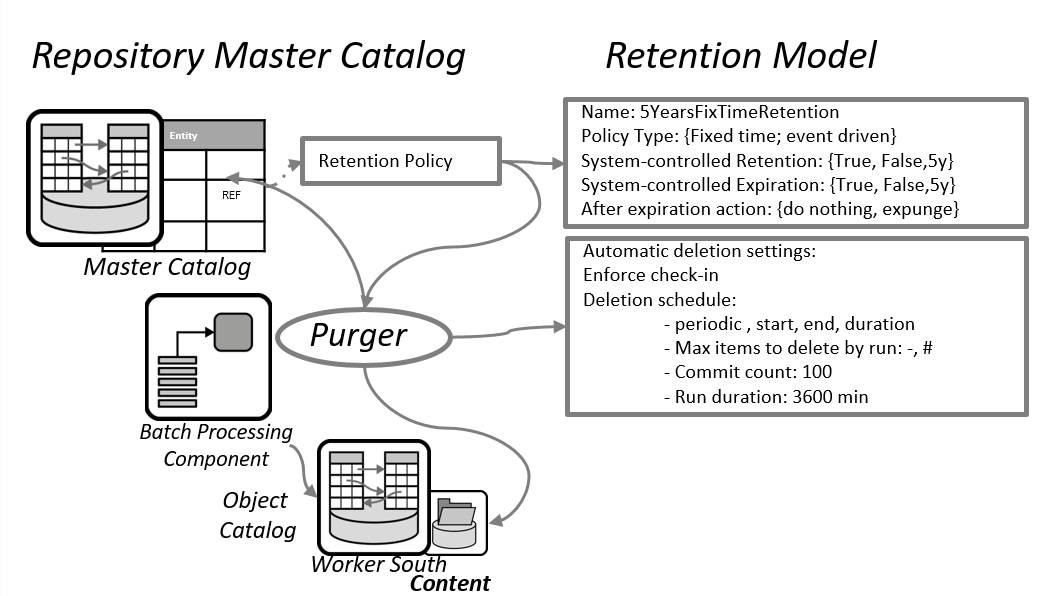
\includegraphics[width=0.5\textwidth]{pics/ECMpic10}
	\caption{Repository support structure for managing retention policies}
	\label{fig:ecm-management}
	\end{centering}
\end{figure}

    \paragraph{} From an ECM system solution standpoint, there exist an integration point with external records management system, representing the authoritative source of the classification, retention and security rules. The integration between the two systems requires the use of specialized software connectors through which the records classification taxonomy and disposition rules are pushed down to the repository and its proper execution is audited and monitored.
    
    \item •	Content centric workflows and document routing support services – relates to a special type of workflows based on routing content triggered by content state changes. The major difference between content-centric and BPMN workflow models is that in the BPMN world the workflow is driven by a control workflow logic that does not depend on the document state or content data, where as in the ECM world the workflow is fully dependent of the state of the content data. A good example is the workflow related to a loan application process in a bank.

\begin{figure}[hbt!]
	\begin{centering}
%	
\includegraphics[width=0.5\textwidth]{logoEC}
	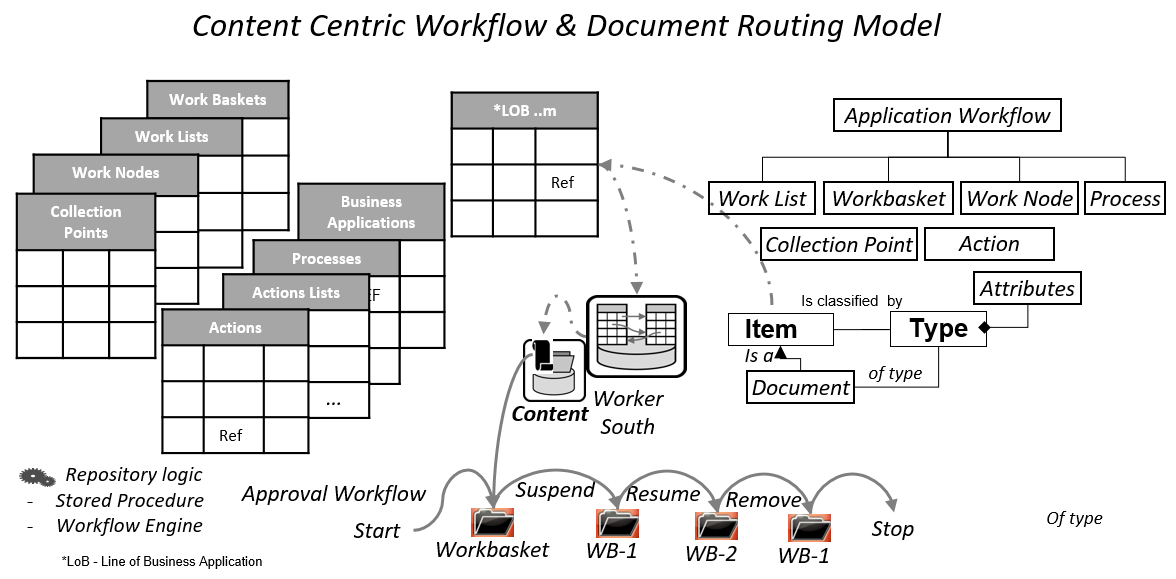
\includegraphics[width=0.5\textwidth]{pics/ECMpic11}
	\caption{Content centric workflow and routing services}
	\label{fig:ecm-workflow}
	\end{centering}
\end{figure}

    \item •	System administration and management services – are the facilities implemented for the administration of ECM systems.

\end{enumerate}

\paragraph{} These services include the definition of administrative domains used to separate tenants and allowing the granting tenants domain specific administrative control. This includes specifying users, groups their roles, privileges and permissions as well as business creating entities and business integration models. Other aspects of system administration are authentication, authorization and access control paired with security \& privacy settings and their enforcement. Governance support is given with the ability to define retention, hold (lock \& unlock) archive and disposition services

\paragraph{} System management provides key features such as the necessary framework for auditing, retention, server management like the content repositories and search/index-server with their associated network communications protocols and the management of the storage server and storage class hierarchies.

\subsection{Resource management services layer }
ECM Resource Managers are responsible for managing the associated content repositories. The number and the locations of resource managers used depends on different factors like: end-user work locations, jurisdictions, quality of service, cost and others. This means resource managers are placed in geographically dispersed location at a branch office or a secondary site. Resource Managers are administered in-dependently. They are responsible for managing the storage devices used for storing the content objects.

\paragraph{} Resource managers have the following sub-components:  

\begin{itemize}
    \item •	Object catalog and content life cycle services 
    \item •	Resource administration and object management services
    \item •	Storage sub-system access and communication services
\end{itemize}

    \paragraph{} The master catalog is in control of the content objects that Resource Managers man-ages when stored on their locally attached storage devices. Object management consists of ensuring that an object is always accessible and retrievable. Objects are mi-grated through a storage hierarchy based migration policies or migrated to other Resource Managers. Objects re replicated, encrypted, rendered into different formats and purged based on retention expiration time. Object access methods vary based on storage device type and access protocol supported.
    
    \paragraph{} The whole dimension of resource and object management is visualized in figure 14 down below.

\subsection{ ECM system component model}

Figure 15 outlines the typical system component model laid out by the ECM system layers as discussed in the previous sections.

\begin{figure}[hbt!]
	\begin{centering}
%	
\includegraphics[width=0.5\textwidth]{logoEC}
	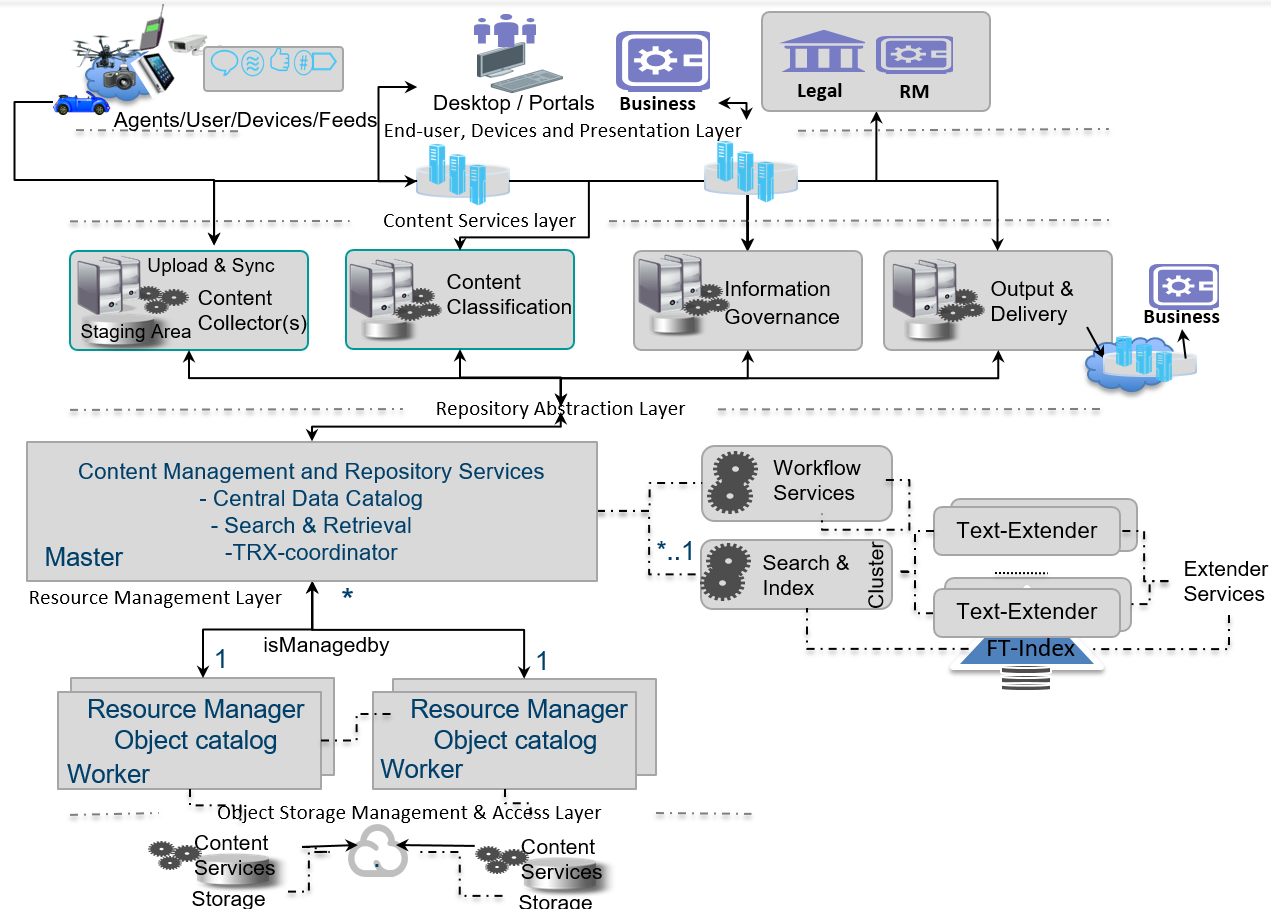
\includegraphics[width=0.5\textwidth]{pics/ECMpic15}
	\caption{ECM system component model}
	\label{fig:ecm-model-componets}
	\end{centering}
\end{figure}

    \paragraph{} In the middle of figure 15 above you can see the single master node and below one to many worker nodes building a multi-level hierarchy. As indicated in the figure 15  master and worker nodes i.e. the central repository and decentralized Resource Managers might result in a deployment topology consisting of a number of heterogeneous, geographically distributed content repository on the server side and a number of repository interface nodes on the client side. Thus, we end up with several flavors of system nodes that is i) the master catalog server node, ii) the search \& index server nodes, iii) one or more content repository server nodes and on the client side  iv) one or more client interface nodes. 

\paragraph{} The different nodes having the following key characteristics: 

\begin{enumerate}
    \item Repository access nodes do host at least the repository APIs be it the custom, standard or federation version. 
    \item The master catalog node functions as the central repository and control server. 
    \item  The search and indexing nodes represent search and retrieval extender nodes building an index cluster  
    \item The worker nodes functions as the physical content repositories the system Object Servers and Resource Managers 
\end{enumerate}

\subsection{ECM system legacy deployment model}

    \paragraph{} In the client-server computing model, the standard way to deploy an ECM system is to design and develop system components as Java EE applications, hosted and running in a Java Web Application Server. The standard access protocols are Https, Web/ REST Services or RPC calls. The application nodes running the software are dedicated physical workstations, virtual machines and lately containers. Most legacy ECM system use dedicated physical machines with dedicated storage and network infrastructure.

\begin{figure}[hbt!]
	\begin{centering}
%	
\includegraphics[width=0.5\textwidth]{logoEC}
	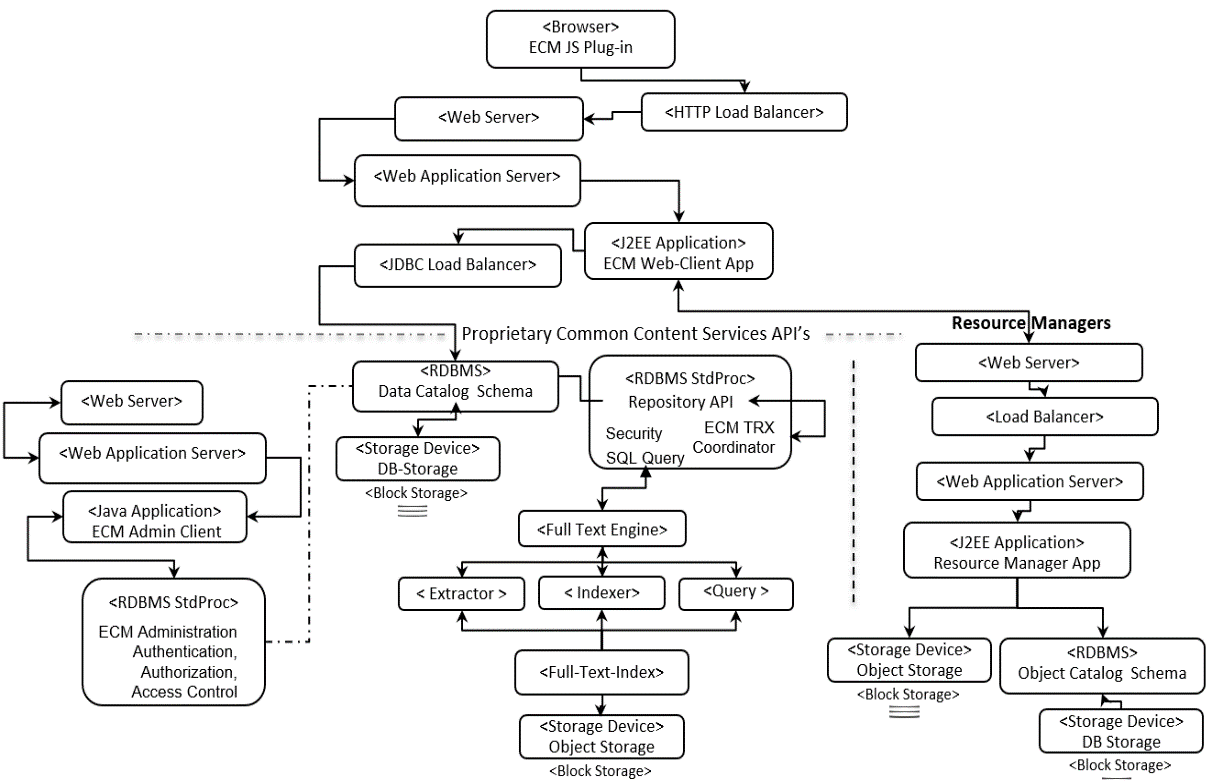
\includegraphics[width=0.5\textwidth]{pics/ECMpic16}
	\caption{ECM system deployment model}
	\label{fig:ecm-model-deployment}
	\end{centering}
\end{figure}

    \paragraph{} The database nodes hosting the system catalog services, due to performance reasons run on dedicated physical machines and some in virtual machines. Usually, data base nodes use dedicated storage and network infrastructure.  In the above topology diagram, you can observe a recurring topology pattern consisting of Web-Server, Load-Balancer, Web-Application Server (WAS), Load-Balancer, Application Component, and Load-Balancer. At the lowest level, you can see the Database Server or the Storage System.  

    \paragraph{} These are some of the components analyzed, and where we found impediments to a smooth deployment onto cloud platforms but also a way to overcome these obstacles. 

\subsection{ECM system implementation model}

    \paragraph{} Figure 17 shows a typical ECM production environment not only meant to deliver the repository services but also to provide a highly available service (HA) that is resilient to system outages due to the presence of a disaster recovery site (DR). This is the reason for triple redundant components at machine, storage and network level.

\begin{figure}[hbt!]
	\begin{centering}
%	
\includegraphics[width=0.5\textwidth]{logoEC}
	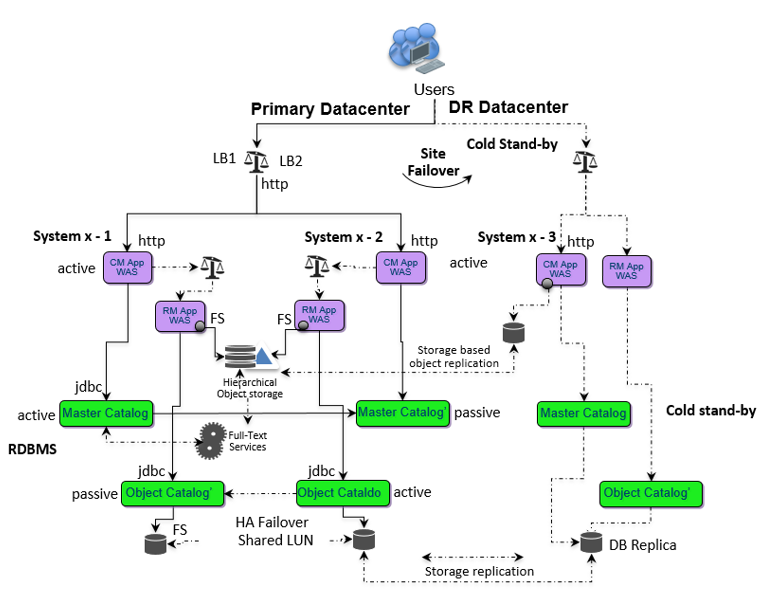
\includegraphics[width=0.5\textwidth]{pics/ECMpic17}
	\caption{ECM system physical implementation model}
	\label{fig:ecm-model-implementaion}
	\end{centering}
\end{figure}

    \paragraph{} As you can see, in figure 17 we outlined two data centers and a component that triggers a site fail-over in case the primary data center stops working due to planned or unplanned outage. The legacy design needs to cope with such an event DNS names and server IP-addresses must change. Going down on the primary site, user traffic hits the load-balancer, typically implemented as redundant physical appliance. The configuration of the load-balancer requires knowing the list of top level of ECM client-application access nodes, their host names and IP-addresses; this is the top-level cluster configuration. The access nodes in turn host a Web-Application Servers (WAS) plug-in that is cognizant of the number of Web-Application Servers, their names, IP-Address and the hosted ECM Java EE applications to which the end users functions calls gets redirected. One level further down the Web-Application Servers (WAS) require a redundant way to connect to the database and the storage systems. 

\section{ECM system prototype implementation and comparison}
\label{sec:prototype}
\subsection{ ECM legacy prototype system}

\paragraph{} The old way of system installation, configuration and deployment

\begin{itemize}
    \item •	Installation prerequisite
    \begin{itemize}
        \item Hardware: Workstation, hard disk, network, IP-Traffic Load Balancer appliance
        \item Co-requisite Software components: Database, Web Application Server, Web Server
        \item ECM Software components: ECM server, ECM API’s, ECM Web-Client Application, ECM Administration Client Application 
    \end{itemize}
    \item •	ECM Configuration and Deployment 
\end{itemize}

\subsection{ECM cloud enabled prototype system }

The new cloud-enabled way of system installation, configuration and deployment

\begin{itemize}
    \item Installation prerequisite
    \begin{itemize}
        \item Hardware: Workstation, hard disk, network, IP-Traffic Load Balancer appliance
        \item Co-requisite Software components: Database, Web Application Server, Web Server
        \item ECM Software components: ECM server, ECM API’s, ECM Web-Client Application, ECM Administration Client Application 
    \item ECM Software components: ECM server, ECM API’s, ECM Web-Client Application, ECM Administration Client Application 
    \item ECM Configuration and Deployment
    \end{itemize}
\end{itemize}

%--------------------------------------------------------------------------------------------------
\section{ECM systems design analysis and results}
\label{analysis_and_results}
 
The legacy design analysis conducted has surfaced the following shortcomings and gaps.  The biggest lesson learned is the fact that in the past, the IT-Infrastructure was lacking many of today functions and features requiring that system design and implementation to fill the gaps at both hardware and software level: The result was application overloaded with operational logic that over the years has become an unnecessary burden.

\begin{figure}[hbt!]
	\begin{centering}
%	
\includegraphics[width=0.5\textwidth]{logoEC}
	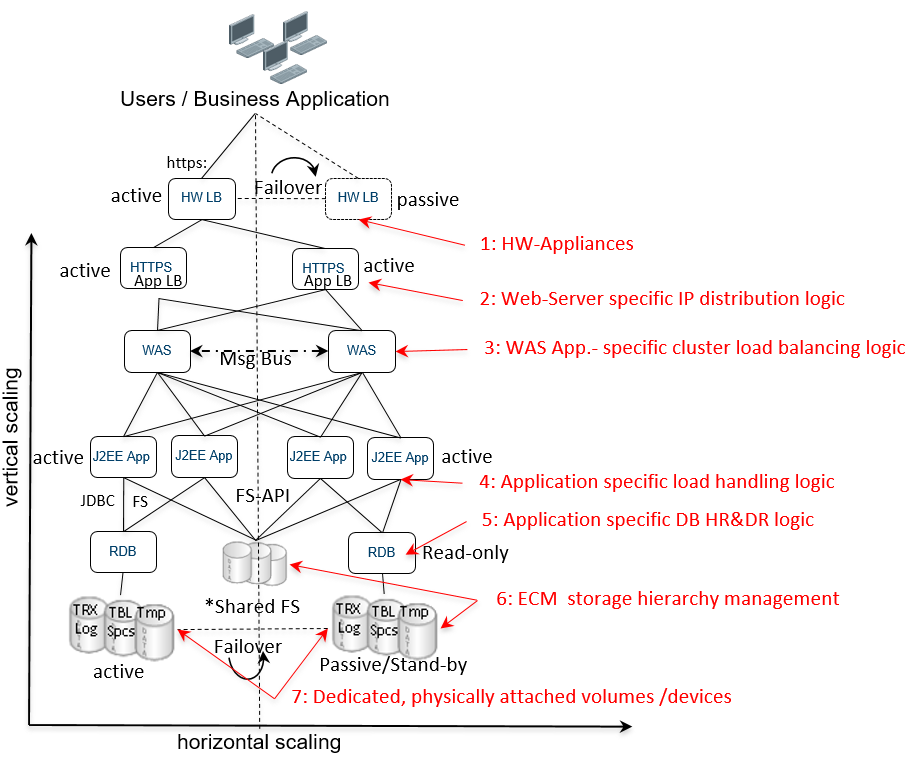
\includegraphics[width=0.5\textwidth]{pics/ECMpic18}
	\caption{ Critical areas of legacy ECM systems components}
	\label{fig:ecm-critical-areas}
	\end{centering}
\end{figure}

    \paragraph{} Therefore, our first conclusion is to decompose the monolithic ECM solutions in to smaller self-sufficient components in order to increase the component autarchy level.

    \paragraph{} Using figure 12 as a reference point and starting from the top we found that 

\begin{enumerate}
    \item Avoid the use of load-balancer hardware appliances and dedicated hardware appliances in general. Use their virtual software defined counterparts instead.
    \item Avoid Web-Server plug-ins configured with application specific logic used for traffic shaping or similar services, if external entities provide those services using a declarative template definition, instead of using custom developed logic.
    \item Web Application Servers tend to implement their own cluster management logic, interfering with external cluster managers and orchestrator tasks preventing a collision free operational co-existence.  
    \item Web Application Servers tend to implement their own redundant JDBC database access that, if monitored and managed from the inside preclude external global cluster activities.    
    \item Revised and adjust the database high availability (HA) and disaster recovery (DR) strategies for running in cloud environments. Database data replication and recovery requires different mechanism when initiated from within a moving container.
    \item Traditionally ECM systems manage the movement of content object through a de-fined storage hierarchy themselves. Equivalent services as provided by modern storage system their use allows to trim down the custom application logic.        
    \item  Finally, we observed that dedicated, physically attached volumes or devices re-quire manual intervention for implementing hardware changes, resulting in system down times and preventing automation.
\end{enumerate}
% ------------------------------------------------------------------------------------------------  

\section{ECM system prototype implementation and comparison}

This section is intended for 

%------------------------------------------------------------------------------
\section{ECM systems design analysis and results}
\label{sect:analysis-results}

%------------------------------------------------------------------------------

\section{Conclusions and outlook}
\label{conclusions}

This paper is the result of our research work around the topic on how to evolve the architecture design of legacy enterprise content management systems for being able to exploit cloud technologies. 

\paragraph{} The legacy ECM architecture design employs a client-server computing model, and design analysis surfaced a number of design shortcomings and gaps because of the paradigm change that happened during transition from client-server to a cloud-computing model. Our observation is that valid design patterns in the one context become design anti-pattern in the other context. These facts prevent that legacy systems run properly in a cloud context. 

\textbf{The key takeaways are:}

\begin{itemize}
    \item 
    \item •	Several of the legacy component come overloaded with application logic that shines through several layers thus preventing a divide and conquer approach. It is necessary to refactor these components into as small as possible self-sufficient sub-components such as to fit into a container running independently in a state less fashion. 
    \item •	Legacy Web-Application Servers come with application logic designed to manage application level topologies of the constituent components as well as application function-call traffic. This type of resource orchestration is no longer necessary at component level and has to be delegate the cloud orchestration services using predefined ECM specific deployment templates. 
    \item •	Avoid the use of hardware appliances, use programmable software components instead, where possible. As an example, use Software Defined Network (SDN) service provided by the cloud platform for load balancing and traffic flow virtual appliances.
    \item •	Avoid the use of physical network and storage links between components, as by doing so moving component transparently in an automated fashion becomes impossible.
    \item •	In the past network and storage devices were dedicate and physically connected to the system components. Today the use of Software Defined Infrastructure (SDI) services is advisable. Declare what is required and leave the actual resource pro-visioning to the cloud platform service.   
\end{itemize}

\paragraph{} This work is the first step to cloud enable ECM systems. It outlined a possible evolutionary path in to the cloud where a CMaaS platform, setup as a self-service offering, running on private and hybrid cloud platform seems very feasible. The good news is that removing the design and implementation shortcomings is possible and closing the gaps looks promising.  We will show how and prove it with a prototype implementation with our next paper. 
%----------------------------------------------------------------------------------------
\section{Future Work}
\label{sect:future-work}

\paragraph{} We plan to further strengthen the..  and promote it for  electronic publishing for  conferences and workshops, and take over the world, as shown in Figure~. We aim at creating a new model of \emph{affordable publishing}, where anybody can become a low-cost publisher. The ... 

%------------------------------------------------------------------------------
\section{Acknowledgments}
\label{sect:acks}

\begin{itemize}
    \item Gang,Shao for the great work he has done in his master thesis and the first prototype   website~\cite{gang-shao}.
    \item .... The University of Manchester) for implementing title-related commands.
\end{itemize}


\label{sec:bib}
\bibliographystyle{plain}
%\bibliographystyle{alpha}
%\bibliographystyle{unsrt}
%\bibliographystyle{abbrv}
\bibliography{ecmbib}

%-------------------------------------------------------------------------------

\appendix {Appendix}

%------------------------------------------------------------------------------
% Index
%\printindex

%------------------------------------------------------------------------------
\end{document}